\chapter{Modeling of Train Operations}
\label{chap:ModelingOfTrainOperations}
\par\noindent
\emph{\textbf{Introduction}} As has been noted in \ref{sec:Solution}, it is necessary to model the braking process of freight trains. All modeling work has been performed with Matlab Simulink. 

\section{Initial Model}
\label{sec:InitialModel}
\par\noindent
The initial model to be expanded upon describes a single braking process. It's sole input, apart from some constants, is pressure over time, meaning a distinct value ranging between 5 and 3.5 bar for every timestamp. For visualization, please refer to \ref{fig:initmodel_siminput}. Let's take a look at the whole model first. 

\begin{figure}[H]
	\centering
	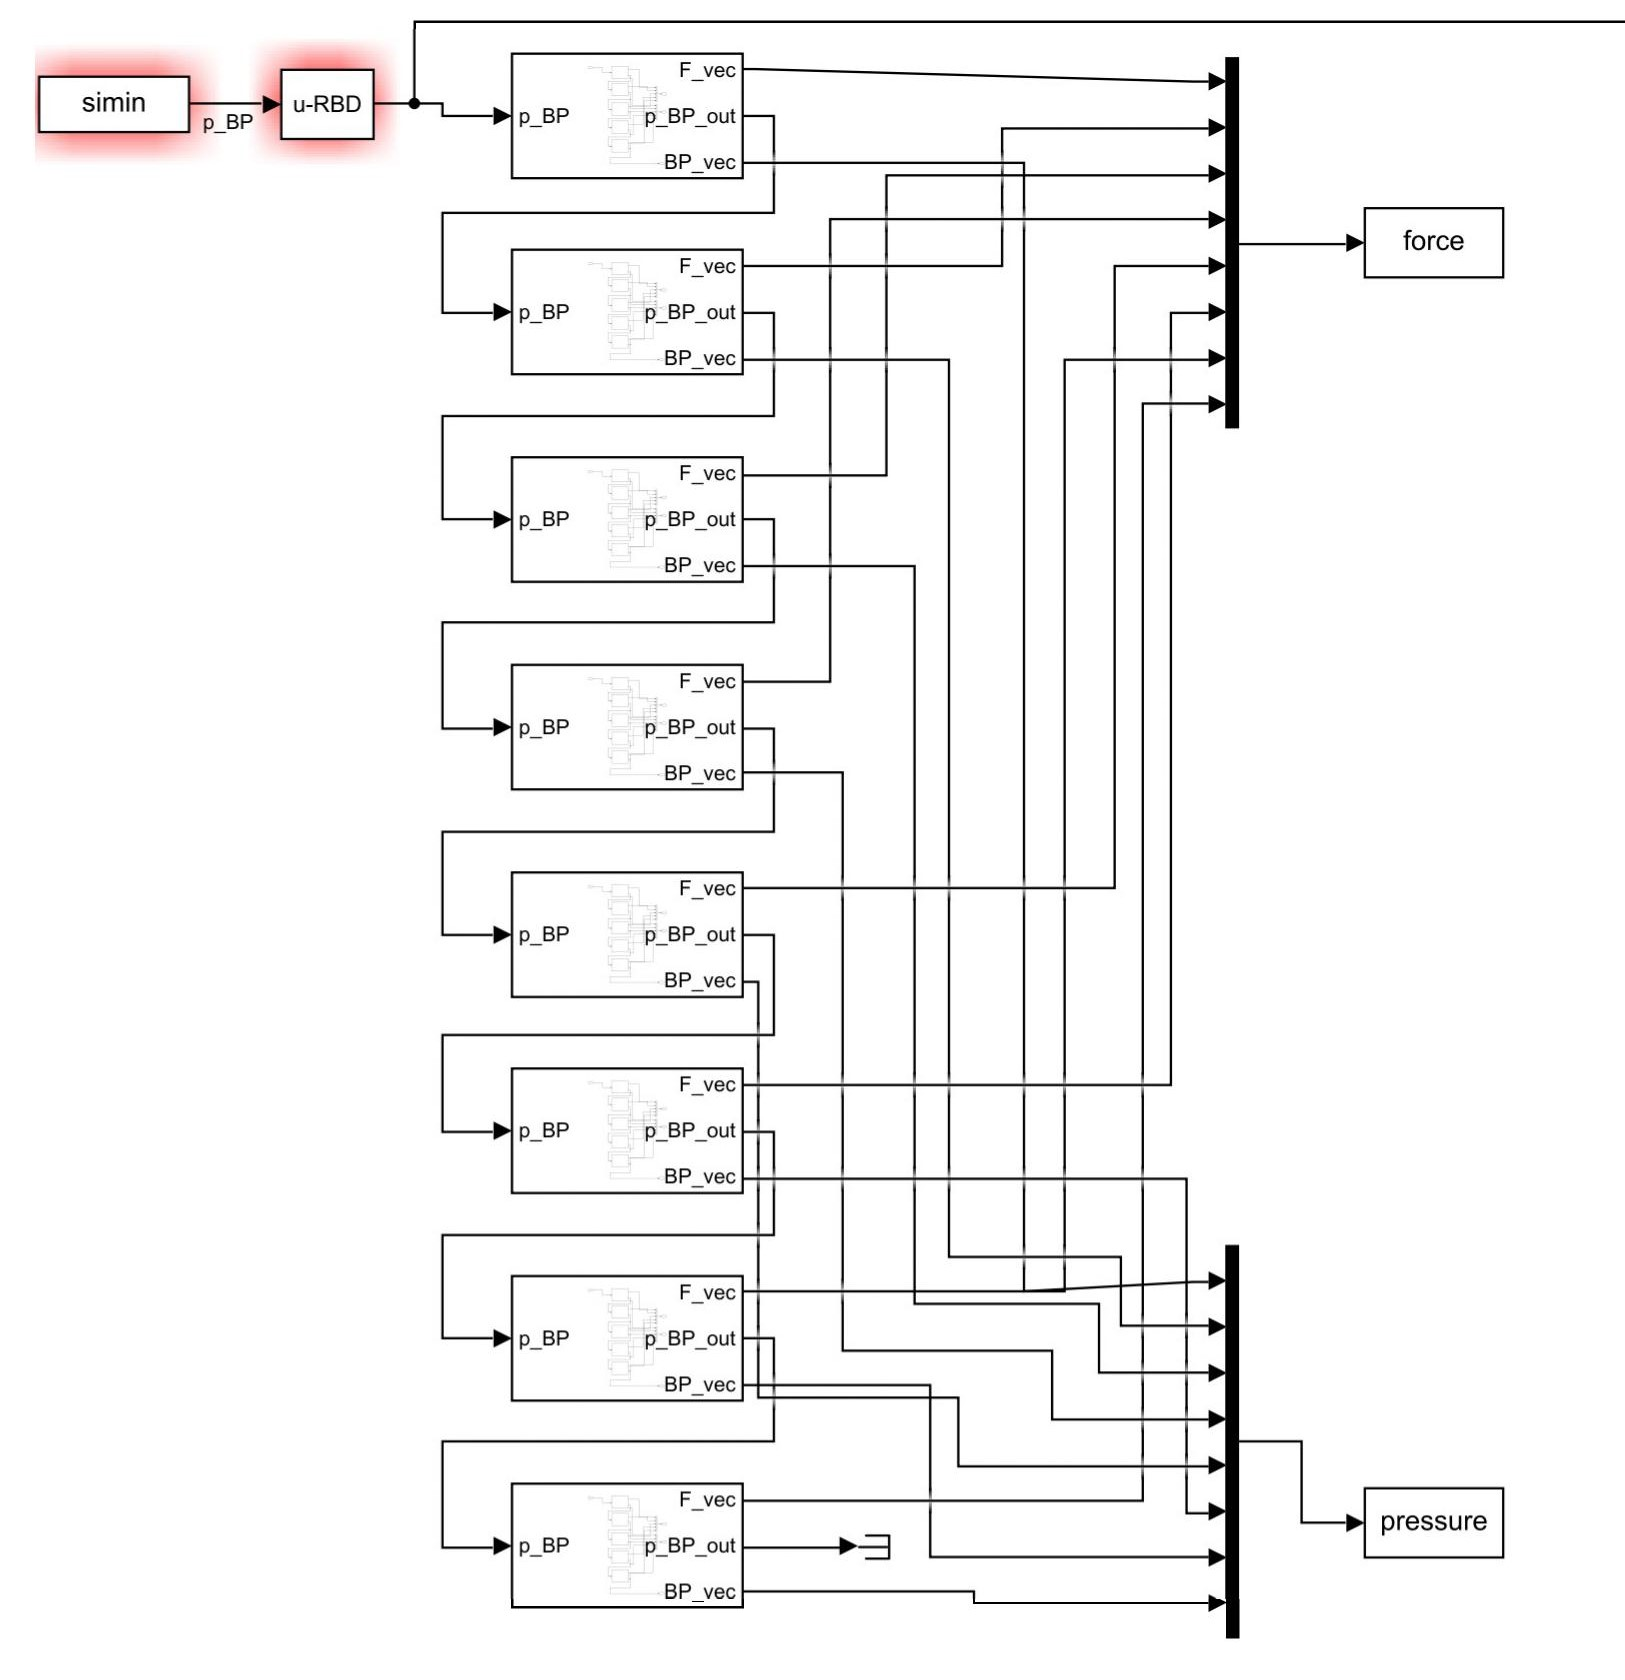
\includegraphics[width=\linewidth]{./pic/initmodel_whole}
	\caption{Initial Model}
	\label{fig:initmodel_whole}
\end{figure}

\par\noindent
Here we see a model of a freight train of fixed length, consisting of 40 wagons, which are, for better readability, further condensed to subsystems of five wagons each, so there are eight of these subsystems. They are interconnected via braking pipe, which is also the sole input to each system. Outputs are braking pressure and braking force. We will take a look at the actual wagon model next.

\begin{figure}[H]
	\centering
	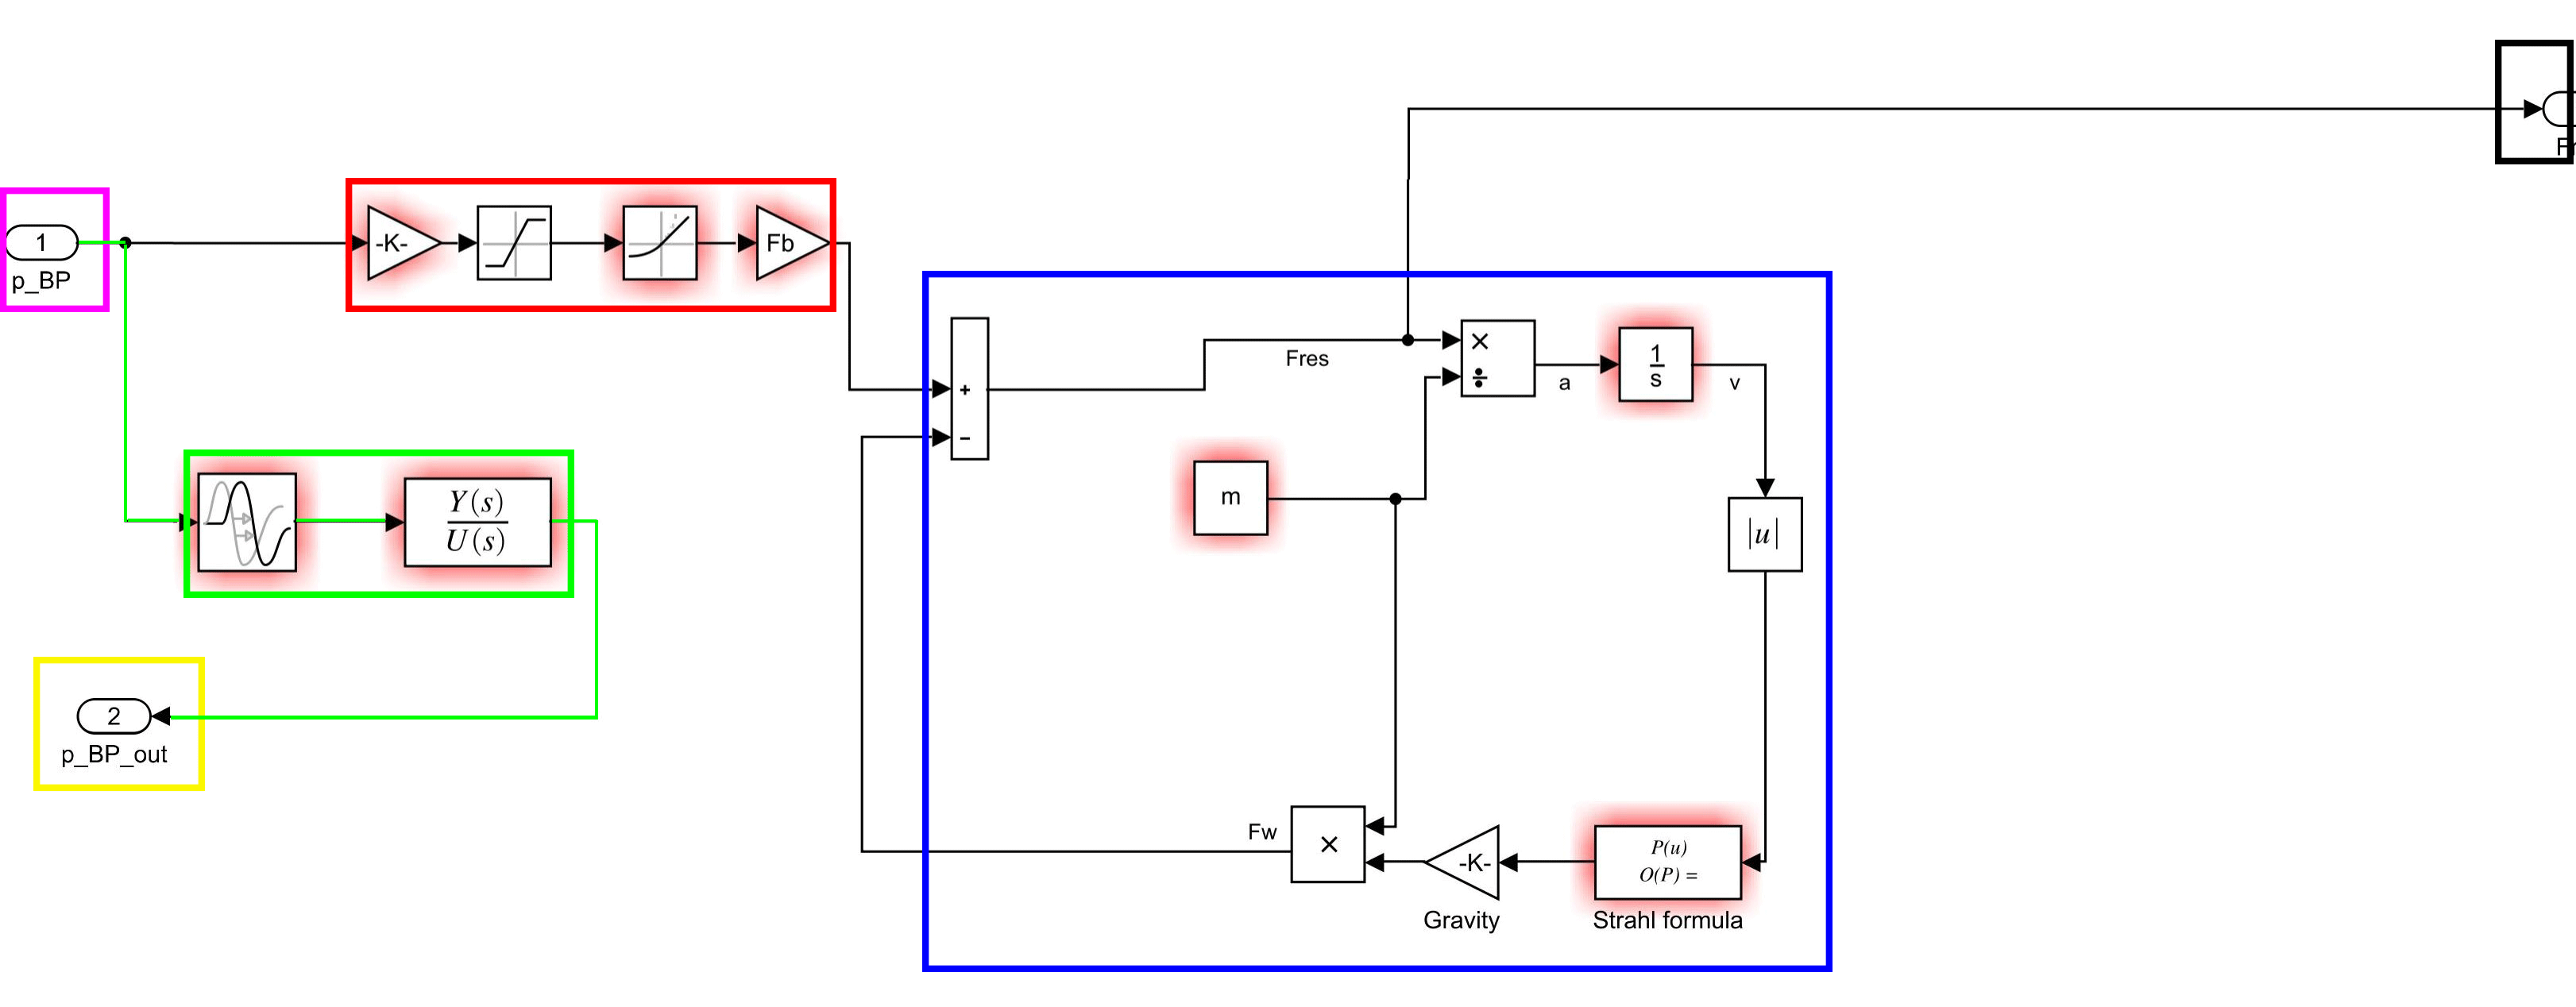
\includegraphics[width=\linewidth]{./pic/initmodel_wagon}
	\caption{Initial Model - Wagon}
	\label{fig:initmodel_wagon}
\end{figure}

\par\noindent
Above is the initial wagon model. \NOTE{All 40 wagon models are identical here. This will be addressed in section \ref{sec:ModelExpansion}}. It consists of three main components.
\par
In the upper left corner is the input, which is the current pressure in the braking pipe. In the lower left corner, the propagation delay of the braking pipe is calculated. This is done by \TODO{}. Top center describes the calculation of the actual braking force, which is achieved by \TODO{}. Finally, the \TODO{Formulieren: Fahrzeugwiderstand}.

\section{Model Expansion}
\label{sec:ModelExpansion}

\par\noindent
This initial model is however not of sufficient detail. Where it merely describes one single braking process, we need to simulate a whole ride, with alternating phases of braking and accelerating. For that purpose, the simulation input has to be adjusted accordingly. Where previously it was only one braking process, using braking pressure as input was the obvious choice, whereas now the idea is to use a kind of track profile, which shall describe the maximum allowed velocity over time, of a notional track. For visualization, please refer to \ref{fig:expandedmodel_siminput}. The simulation then only needs to brake or accelerate depending on train velocity versus maximum velocity at the current time.

\par
Accordingly, the first expansion step is to create a mechanism to control the train so to speak. For this purpose, the system simply checks for each timestamp whether the current velocity of the train is greater than the maximum allowed velocity at the current time, according to simulation input. If this is the case, a braking pressure is applied to the pipe, scaling with the difference between $v_{max}$ and $v_{real}$, $v_{dif}$. This means the higher $v_{dif}$ is, the more braking pressure gets applied. This more or less covers the braking part of the system.

\par
The model however also needs a component for acceleration. To simplify things, the logic here is that if the train is not braking, it is accelerating, which actually works out pretty well. To accelerate, a traction force is applied, which also scales with $v_{dif}$, so the higher $v_{dif}$, the higher the applied traction force.

\begin{figure}[H]
	\centering
	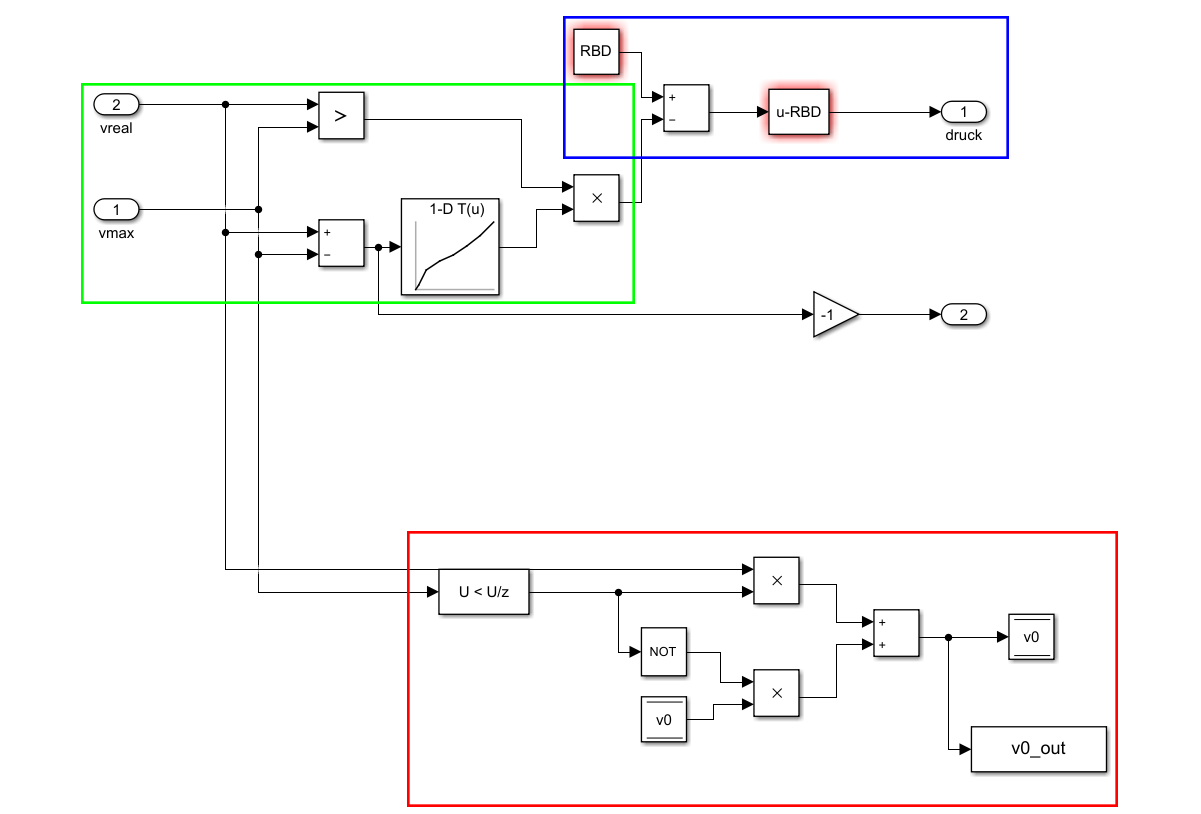
\includegraphics[width=\linewidth]{./pic/expandedmodel_pressure}
	\caption{Expanded Model - Pressure Calculation}
	\label{fig:expandedmodel_pressure}
\end{figure}

\par\noindent
Depicted above is the system which determines braking pressure to apply. It calculates $v_{dif}$ by subtracting $v_{max}$ from $v_{real}$, which is then fed into a one-dimensional lookup table. The table is a sampled representation of a function with fixed breakpoints, mapping one function value to each breakpoint, like so

\begin{equation}
\label{eq:lookuptable}
H(n) =
\begin{cases}
0.1 & \text{if $n=1$} \\
0.7 & \text{if $n=15$} \\
0.8 & \text{if $n=20$} \\
\text{..}
\end{cases}
\end{equation}

\noindent
where $n$ is the breakpoints of $v_{dif}$. Since the pressure should only be applied if $v_{real}$ is greater than $v_{max}$, the ultimate result follows the logic of the following equation

\begin{equation}
\label{eq:brakingpressure}
P(n,t) = H(n) * (v_{real}(t) > v_{max}(t))
\end{equation}

\noindent
where $v_{real}(t)$ is train velocity over time, $v_{max}(t)$ is maximum velocity over time, and $v_{real}(t) > v_{max}(t)$ is either 1 or 0.

\begin{figure}[H]
	\centering
	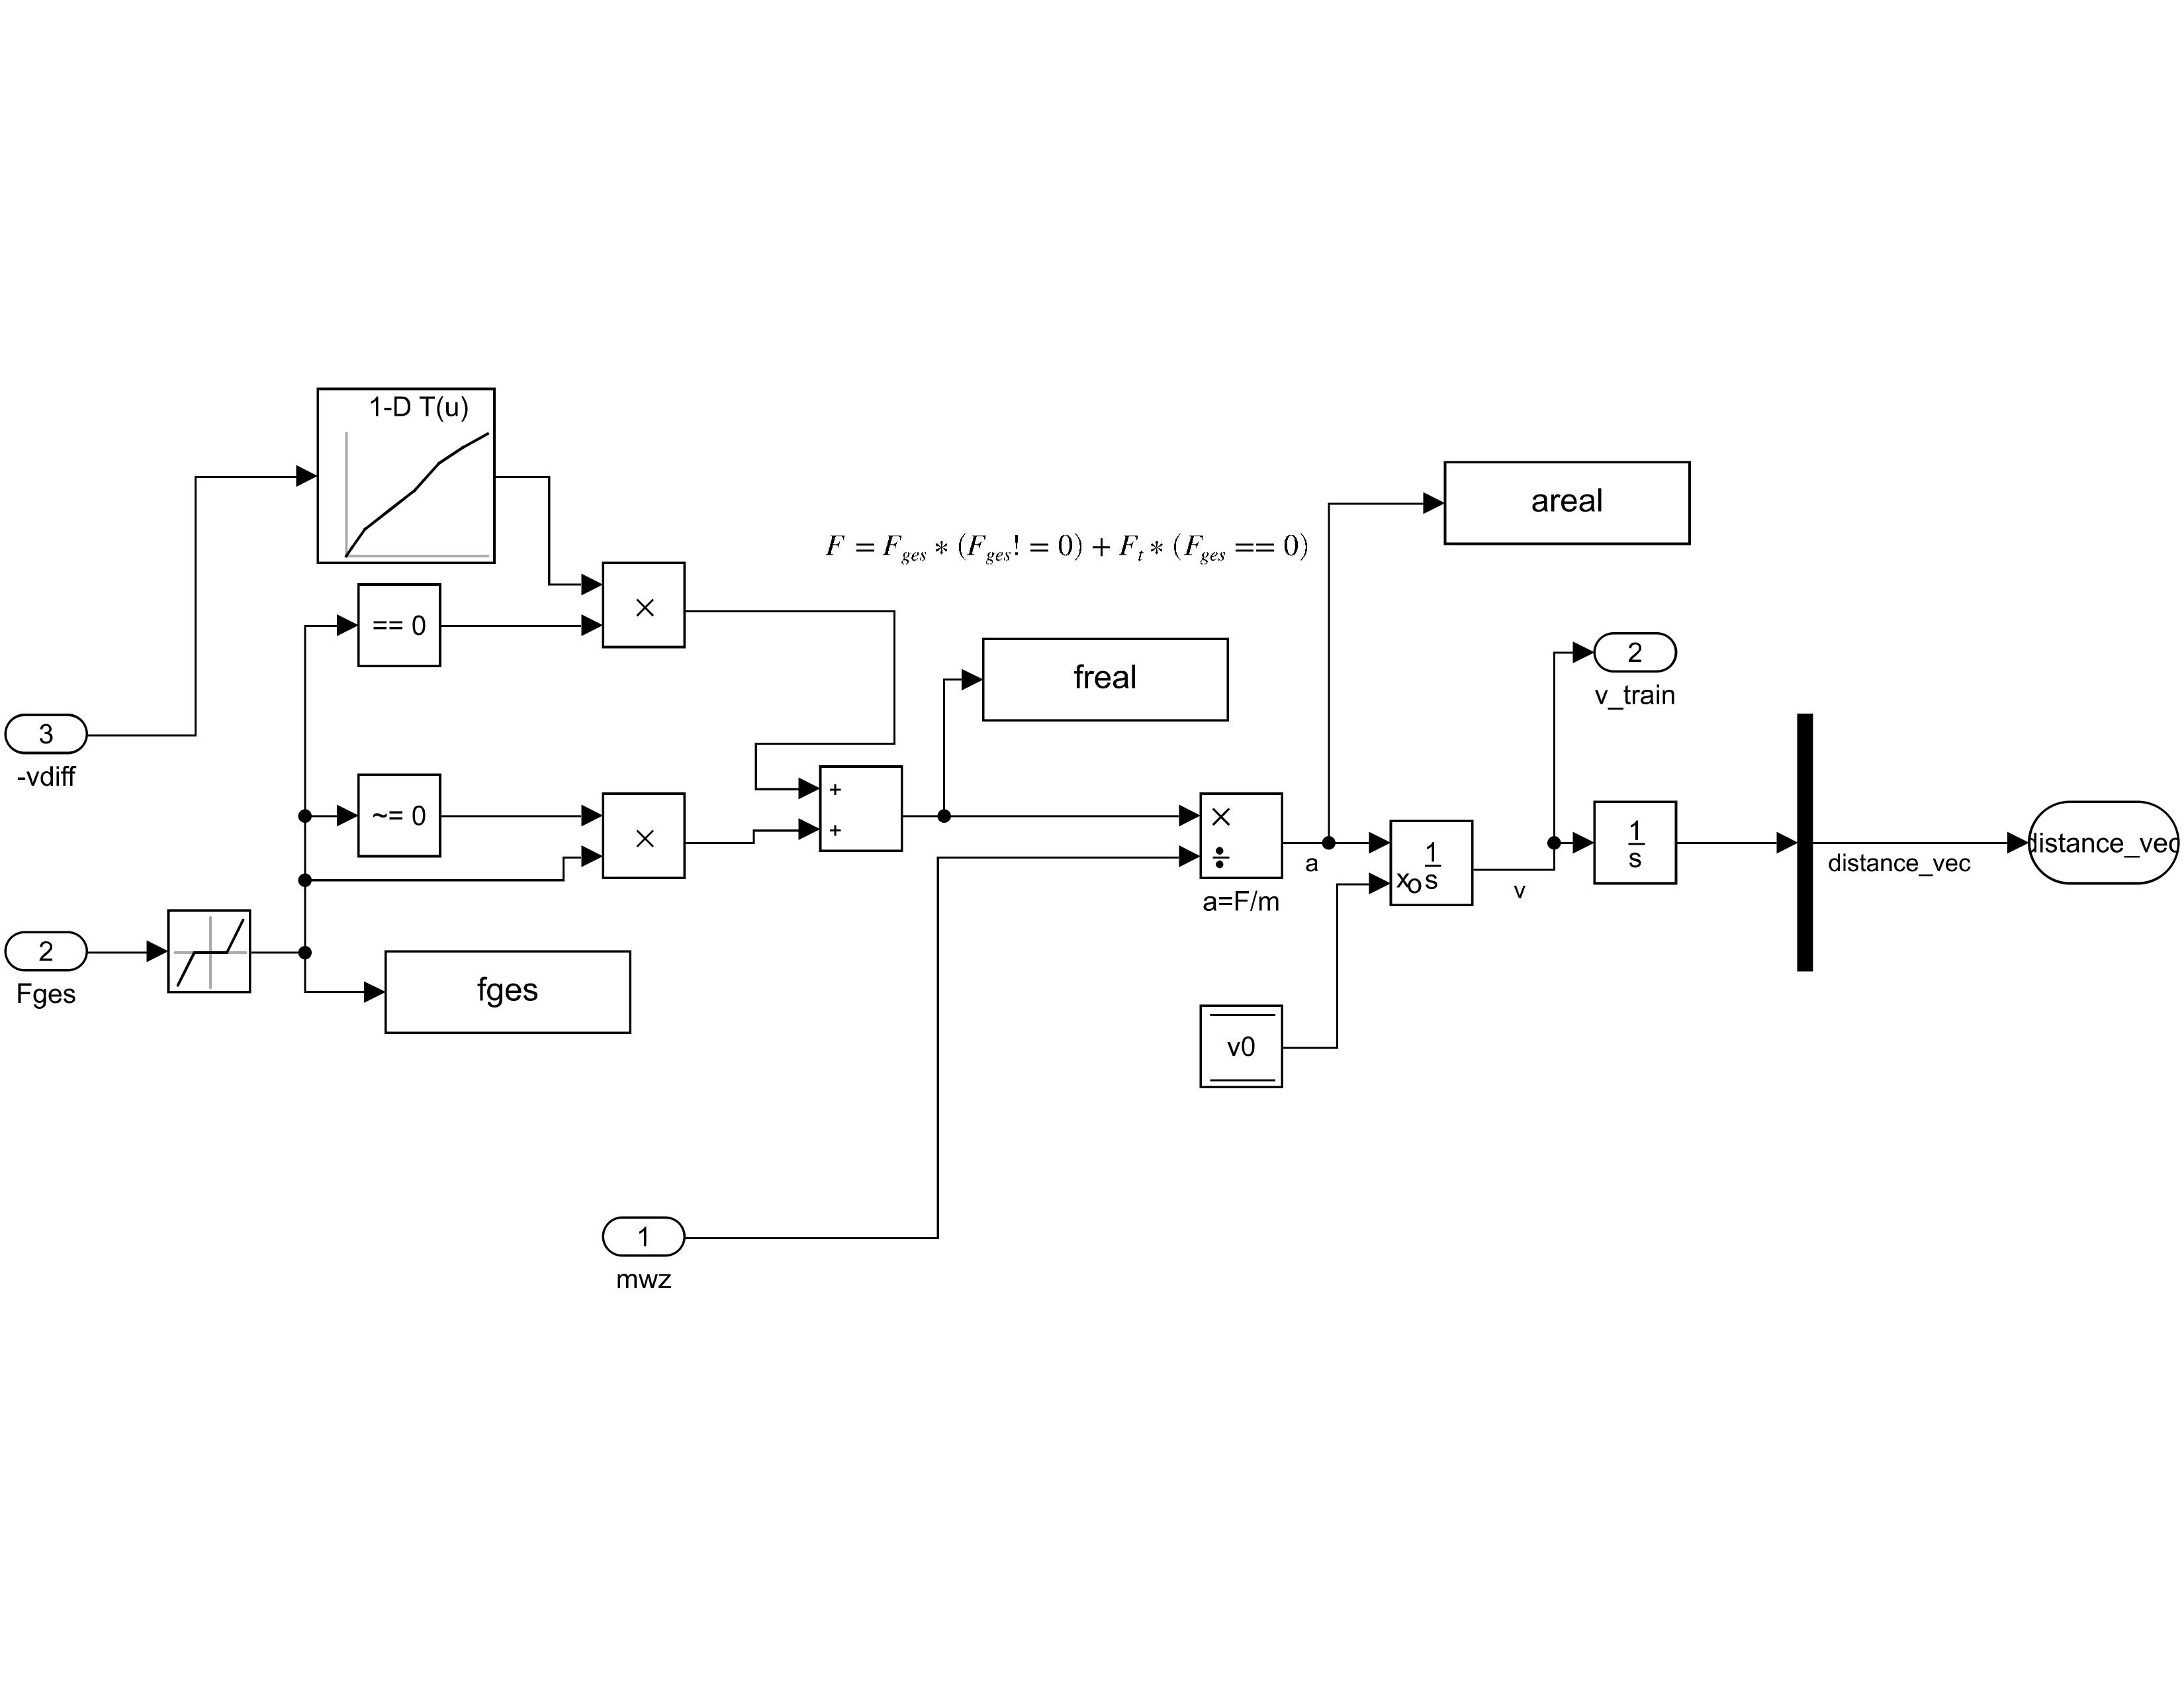
\includegraphics[width=\linewidth]{./pic/expandedmodel_force}
	\caption{Expanded Model - Traction Force Calculation}
	\label{fig:expandedmodel_force}
\end{figure}

\par\noindent
The above system determines the traction force to apply. As has been discussed earlier, this works like a simple bang-bang controller. The design is very similar to the braking pressure system: $v_{dif}$ is again fed into a one-dimensional lookup table, which outputs different values for traction force accordingly. The higher $v_{dif}$ is, the higher the traction force to apply. It is then added to the current braking force, however only either traction or braking force is at any given time positive while the other is zero, which is achieved by the equations
 
\begin{equation}
\label{eq:tracforce}
f(n,t) = H(n) * (F_{B}(t) == 0) 
\end{equation}

\noindent
where $n$ is $v_{dif}$, $H(n)$ is the lookup table function (see equation \ref{eq:lookuptable}), $F_{B}(t)$ is the braking force over time, and 

\begin{equation}
\label{eq:brakeforce}
g(t) = F_{B}(t) * (F_{B}(t) \neq 0)
\end{equation}

\noindent
where $F_{B}(t)$ is the braking force over time, so we have 

\begin{equation}
\label{eq:force}
F(n,t) = f(n,t) + g(t) 
\end{equation} 

\noindent
where $F$ is the actual force over time, either braking or traction.

\par\noindent
$F$ is then used to calculate acceleration. According to Newton's Second Law,
\begin{equation}
\label{eq:newton}
F = m * a
\end{equation}
Accordingly, acceleration is
\begin{equation}
\label{eq:acceleration}
a = F(n,t) / m
\end{equation}
	
\noindent
where $m$ is the accumulated mass of all wagons and $F(n,t)$ relates to equation \ref{eq:force}. The acceleration is then used to calculate the velocity by integrating $a$ in relation to $v_{0}$, which is the initial velocity of the current braking or acceleration process \TODO{überprüfen..}. Integration of $v$ in turn allows calculation of the traveled distance.

\begin{figure}[H]
	\centering
	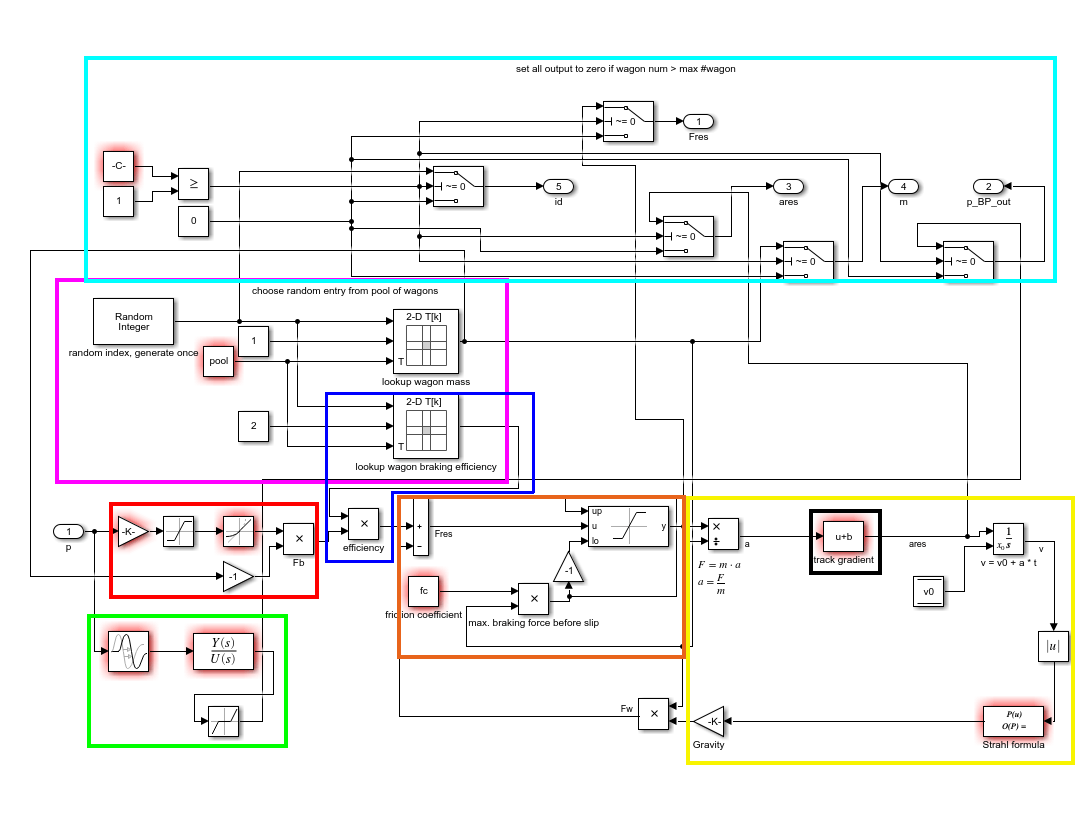
\includegraphics[width=\linewidth]{./pic/expandedmodel_wagon}
	\caption{Expanded Model - Wagon}
	\label{fig:expandedmodel_wagon}
\end{figure}

\par\noindent
The last subsystem is the actual wagon. We will take a look at the largely unchanged elements first. The sole input is still the braking pressure on the brake pipe. Simulation of the propagation delay has also remained the same as before. 

\par
One new addition is a pool of different wagons. Whereas before all 40 were distinguishable only by their position, they are now assigned with different parameters. To that end, a pool of 500 wagons has been randomly generated via python script, where each wagon has a unique ID, as well as randomly generated mass and braking efficiency. In actual simulation, up to 40 of these 500 are, currently by generation of random indices, selected and their properties used accordingly. It would also be possible to determine the wagon ids to be used beforehand, instead of choosing randomly.

\par
Another requirement was to make the number of wagons variable. In the initial model, the modeled train had a fixed number of 40 wagons, therefore also 40 wagon subsystems. Unfortunately, simulink offers no way to disable certain subsystems dynamically, but only by manually turning them off via model explorer, which would be unfeasible for such a large number of simulations. To circumvent this issue, output gets disabled for all unwanted wagons. For a simulation of a train of 20 wagons, the first 20 remain untouched, while the latter 20 produce no output and therefore also have no impact on the overall simulation. The turning off is achieved by simple switches; each wagon subsystem has a unique index from one to forty. If the index is greater than the specified number of wagons, all switches are turned to output zero.
	
\section{Further Expansion}
\label{sec:FurtherExpansion}